%# -*- coding: utf-8-unix -*-
%%==================================================
%% chapter01.tex for SJTU Master Thesis
%%==================================================

\chapter{绪论}
\label{chap:introduction}

\section{引言}
\label{sec:objective}
隐私是一种与公共、群体利益无关,不便或者不愿他人知道的、应予以保密的信息,是不以他人是否承认或评价为转移的存在。
%从人类有意识开始,隐私意识便是最先表现出来的本能特征,伴随着时代文明的发展,人类具有越来越强的隐私保护意识。
“数据时代”的飞速发展使得信息数据的采集、存储和发布变得更加方便快捷,海量数据的处理技术以及数据挖掘、机器学习算法的应用使得数据的共享和学习变得更加高效准确,但与此同时,新的隐私攻击手段、黑客技术也在不断涌现。科技和时代的发展在带给我们高品质生活的同时,数据中的隐私保护问题面临着愈加严峻的挑战。
本课题基于最高隐私保障的差分隐私技术,基于经典的非交互式差分隐私匿名算法,设计对高维度查询应用具有良好扩展性的算法DiffCon,有效提升了发布数据的分析准确度。本章节将简要介绍相关的课题研究背景,
%总结各类隐私保护算法和面向数据挖掘分类问题的研究现状,
归纳课题相关的
%隐私保护算法和分类问题的
研究现状,最后明确课题目标、介绍论文结构。


\section{课题研究背景}

\subsection{隐私及隐私保护}  %隐私的定义,度量,泄露风险及隐私保护研究方向

隐私指的是个体不愿被外界获悉的敏感属性,比如个人的病理特征,资产状况,家庭住址等。隐私分为两类\cite{Defining Privacy for Data}:
\begin{enumerate}
	\item 个人隐私(individual privacy):任何可以直接或间接标识特定人物且不愿被披露的信息,可以是个人的物理信息,生理信息或社会属性信息等。
	\item 共同隐私(corporate privacy):包含了所有人共同的个人隐私的信息,如工厂工人的薪资分布。
\end{enumerate}

隐私的保护程度可以用隐私的“披露风险”(disclosure risk)\cite{l-diversity}来度量,披露风险越高意味着隐私保护程度越低。披露风险是与攻击者所具备的背景知识(background knowledge)相关的\cite{面向数据库应用的隐私保护研究综述},若s表示隐私信息,Pr[E]表示事件E发生的概率,那么在公布背景知识E的前提下隐私信息s披露的风险\textsc{R}(s,E)表示为
\[
	\textsc{R}(s,E) = Pr(E_{s}).
\]
披露风险\textsc{R}(s,E)可以用来度量隐私保护程度,如$l$-diversity算法\cite{l-diversity}保证隐私披露风险不超过1/$l$,$m$-Invariance算法\cite{m-Invariance}的披露风险不超过1/$m$。

隐私保护的研究方向是由具体应用领域的需求来决定。面向数据挖掘类应用的隐私保护技术主要是研究针对某类数据挖掘算法,根据其特性设计出适应性良好的隐私保护算法,如Clustering\cite{clustering}算法;基于数据发布的隐私保护技术,主要是通过泛化或加密技术发布处理后的数据提供给各类应用,如一系列匿名化算法\cite{multidimensional k anonymity};面向分布式环境下的隐私保护技术,如在智能电网中的应用\cite{Distributed Privacy}。

隐私保护手段大体上分为4类\cite{面向数据库应用的隐私保护研究综述}:(1)基于数据失真(distorting)的技术,如通过添加噪音(noise)的方式达到模糊敏感数据的目的,同时保持数据集的统计特征。(2)基于数据加密技术隐藏敏感数据。(3)基于限制发布的保护技术,如泛化数据域。(4)结合以上三种方式的优点生成的新方法。


\subsection{差分隐私背景} %交互和非交互框架,隐私代价分配和消耗 列联表 直方图

$\varepsilon$-差分隐私($\varepsilon$-differential privacy)\cite{Dwork Calibrating}不同于传统的隐私保护技术,它对隐私披露风险给出了严谨的量化证明,并且定义了严格的攻击模式,因此不关心攻击者所获取的背景知识。通过拉普拉斯加噪机制\cite{Dwork Calibrating}设计满足差分隐私定义的算法,就能够给数据提供最高级别的隐私保障力度。$\varepsilon$是隐私预算(private budget),表示隐私的保护程度,$\varepsilon$越小则隐私保护程度越高。
差分隐私技术的研究主要在于两个方面:(1)如何设计满足差分隐私定义的隐私保护算法。(2)如何减少噪音扰动,保证加噪后数据的高可用性。

差分隐私保护框架分为两种:交互式框架和非交互式框架,如图\ref{fig:interactive framework}和图\ref{fig:non-interactive framework}所示。

在交互式框架中,用户提交查询请求给数据库之后,数据库的应答作为某种差分隐私处理算法的输入,返回输出结果给用户。这个过程中差分隐私处理算法成为了用户和数据库之间的查询接口,但经过一定数量的查询之后将耗尽隐私预算$\varepsilon$,此后的查询就不再满足差分隐私定义,因此无法保证隐私安全。

在非交互式框架中,差分隐私算法先处理包含隐私信息的原数据集,发布出安全的新数据集;接着用户采用常规数据库查询操作与新数据集交互,得到请求应答。显然这个离线模式的框架具有诸多优点,并且不存在隐私预算由于过多的查询请求而被耗尽的问题,因此主要的研究点在于优化发布数据的可用性。

\begin{figure}[!htp]
	\centering
	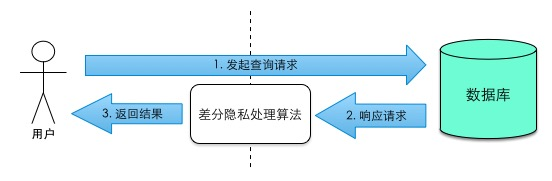
\includegraphics[width=5in]{chap1/interactive}
	\bicaption[fig:interactive framework]{图}{交互式框架}{Fig.}{interactive framework}
\end{figure}

\begin{figure}[!htp]
	\centering
	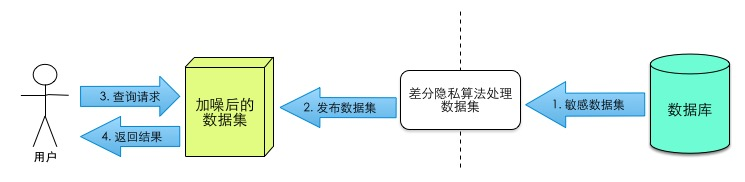
\includegraphics[width=5in]{chap1/non-interactive}
	\bicaption[fig:non-interactive framework]{图}{非交互式框架}{Fig.}{non-interactive framework}
\end{figure}


\subsection{决策树} %主要的数据挖掘分类算法,信息增益,C4.5,CART对于离散和连续属性的处理问题

数据挖掘分类算法是一种监督学习(Supervised Learning)算法,典型代表是决策树模型(Decision Tree)\cite{decision tree},在训练阶段,它通过训练样本集构建树状的分类结构,在每个内部节点做属性选取以及样本分类,最后在叶节点标识类别。在使用中,测试样本集从根节点开始,能在树中找到一段自顶向下的匹配路径并最终落到某一叶节点上,此叶节点即为学习到的类别属性。构建树的过程中属性的选择方式是决策树算法的关键,直接影响到分类性能的好坏。经典的决策树学习算法有ID3\cite{decision tree},C4.5\cite{c45},CART\cite{cart},本小节对ID3和C4.5做简要介绍,并讨论离散属性和连续属性问题。

\begin{exmp}
	S为训练集,S的目标属性C有m个可能的类标号值,C=\{C$_{1}$,C$_{2}$,...,C$_{m}$\},C$_{i}$(i=1,2,...,m)在所有样本中出现的概率为P$_{i}$。有离散属性A可对训练集S进行划分,假定A有k个不同的取值,能把S划分成k个样本子集\{S$_{1}$,S$_{2}$,...,S$_{k}$\},每个子集的样本数为|S$_{j}$|(j=1,2,...,k)。
\end{exmp}
ID3算法用熵(Entropy)来度量一个属性所具有的信息量,熵值越小说明样本对目标属性的分布越纯。熵值的计算为
\[
	Entropy(S) = -\sum_{i=1}^{m}P_{i}\log_{2}(P_{i})
\]
ID3用信息增益(Gain)作为属性选择的标准,训练集S经属性A划分的信息增益计算式为:
\[
\begin{split}
	Entropy_{A}(S) &= \sum_{i=1}^{k}\frac{|S_{i}|}{|S|}Entropy(S_{i})\\
	Gain(S,A) &= Entropy(S)-Entropy_{A}(S)
\end{split}
\]
信息增益越大说明使用属性A划分后的样本子集越纯,越有利于分类。因此,决策树构建过程中,计算所有候选属性的信息增益,选取其中最大的属性。

但是,在ID3算法中可以看到它只能处理离散型属性,若属性A是一个连续型属性,那么单纯通过A在样本中出现的属性值来划分S显然是不合理的。例如A表示人类年龄,若选择了属性A那么S会由于的各种不同的年龄值被分成众多的细小子集,并且大部分子集仅有一条样本,这种分类选择显然不符合实际。对于这个问题,C4.5算法对连续属性提供了良好的支持。

对于训练集S中的连续属性B,C4.5按B的取值进行递增排序,将每对相邻值的中点看成可能的分裂点。对于每个分裂点,根据分裂点的数值对训练集S进行划分,在属性B上小于分裂点值的样本归入左部训练集S$_{L}$,大于的部分归入右部训练集S$_{R}$。那么此分裂点的熵值为:
\[
	Entropy_{B}(S) = \frac{|S_{L}|}{|S|}Entropy(S_{L})+\frac{|S_{R}|}{|S|}Entropy(S_{R})
\]
同理计算所有分裂点的熵值,取最小的一个分裂点作为属性B的最佳分裂点,并且将其熵值与别的属性进行比较从中选择最优属性,从而解决连续属性的熵值计算问题。此外,C4.5还引入了信息增益率(Information gain ratio)来调节信息增益平衡,消除属性取值数目的影响。

对于离散和连续属性的处理以及分裂属性的选择方式是决策树分类问题的重要研究点,在差分隐私技术中还关系到隐私代价的损耗和分布,将在后续章节深入讨论。

\section{相关研究现状} %主要讨论面向分类的差分隐私算法

差分隐私技术的突出优势使它成为了近些年来隐私保护研究的热点,基于不同的应用领域产生了诸多研究方向。接下来就本课题所涉及的方向,分别对匿名化、面向分类应用的隐私保护和维度问题做相关的研究现状介绍。

\subsection{链接攻击和$k$-匿名算法}  %k匿名算法

链接攻击是背景知识攻击\cite{compounding attack}\cite{background attack}的一种常见手段,它通过其他渠道获得的外表与发布的数据表进行链接操作,进而推断出隐私信息。如下图\ref{fig:anonymity1}所示的是一个经过初步处理后发布的的个人信息表——删除能直接标识单一个体的显示标识符(explicit identifier)“姓名”。但是仅仅删除显示标识符是不够的,若攻击者获得外表\ref{fig:anonymity3},进行链接操作之后图\ref{fig:anonymity1}的处理就无法保证隐私安全了——通过“邮编”、“出生日期”和“婚姻状况”的链接,易推得姓名是“小文”以及她的病况。

\begin{figure}[!htp]
	\centering
	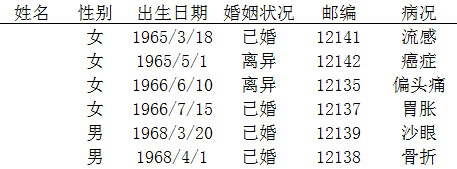
\includegraphics[width=5in]{chap1/anonymity1}
	\bicaption[fig:anonymity1]{图}{隐藏关键属性后的个人信息表}{Fig.}{Personal information form after hiding the key attributes}
\end{figure}

\begin{figure}[!htp]
	\centering
	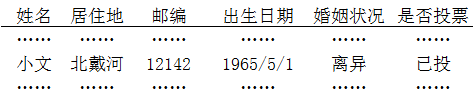
\includegraphics[width=5in]{chap1/anonymity3}
	\bicaption[fig:anonymity3]{图}{投票登记表}{Fig.}{Voting registration form}
\end{figure}


匿名化是隐私保护算法的主要实现技术之一,主要通过“抑制”和“泛化”操作分别达到隐藏显示标识符和抽象敏感属性的保护手段。最具代表性的匿名化算法是L.Sweeney和P.Samarati提出的$k$-匿名($k$-anonymity)\cite{k-anonymity}算法。它定义准标识符(Quasi-Identifies,QI)来表示那些能够与外表进行链接以标识个体身份的属性或属性组合,如表\ref{fig:anonymity1}的属性组{性别,出生日期,婚姻状况,邮编}就是个人信息表的QI。显然,QI的定义是依赖于外表信息的,对于同一个隐私表可能由于不同的外表的存在定义了不同的QI。$k$-匿名算法旨在能够使得匿名处理后的隐私表的每条记录至少与其他$k$-1条记录具有完全相同的QI属性值,那么在链接攻击后得到的元组中,在每个QI属性上至少包含了$k$条相同属性值的记录,因此无法唯一区分个体身份。

表\ref{fig:anonymity2}是对表\ref{fig:anonymity1}进行$k$=2的2-匿名处理后得到的结果,邮编和出生日期基于数值型泛化技术予以抽象处理,用更大的取值范围代替原值。可以看到泛化处理在保护隐私的同时带来了信息的损失,如何减小匿名化算法的信息缺损(information loss)\cite{Bottom-up generalization}\cite{Top-down specialization}成了优化匿名保护算法的一个重要研究点。

\begin{figure}[!htp]
	\centering
	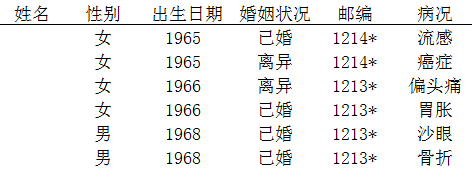
\includegraphics[width=5in]{chap1/anonymity2}
	\bicaption[fig:anonymity2]{图}{2-匿名化处理后的个人信息表}{Fig.}{personal information form with 2-anonymity}
\end{figure}

\subsection{面向分类应用的差分隐私算法}  %firedman

在分类需求的数据挖掘模型中,可以从训练数据中学习到有用的经验规则,但是在分析数据的同时极有可能泄露隐私,结合差分隐私技术给这一领域提供了新的解决思路。

分类模型的典型代表是决策树模型。SuLQ ID3\cite{SuLQ}是基于ID3算法的交互式差分隐私模型,它事先规定了决策树的树高并均分隐私预算到每层,在选择分类属性时通过往熵值添加满足差分隐私的拉普拉斯噪音达到隐私保护的目的。就1.2.3节的例1.1背景,对于有m个类属性C的训练集S,在属性A(有k个属性值)上对其进行划分得到\{S$_{1}$,S$_{2}$,...,S$_{k}$\},在计算信息增益时需要计算S的熵值和由A划分后的熵值。SuLQ ID3在每次选择属性的过程中,对类个数|C$_{i}$|(i=1,2,...,m)、划分后的子集大小|S$_{j}$|(j=1,2,...,k)等数值上添加拉普拉斯噪音,分别得到|$\widetilde{C_{i}}$|,|$\widetilde{S_{j}}$|等加噪结果。下式描述了SuLQ ID3中信息增益的计算,上方带波浪号表示添加了拉普拉斯噪音处理后的结果:
\[
\begin{split}
	En\widetilde{tro}py(S) &= -\sum_{i=1}^{m}\frac{|\widetilde{C_{i}}|}{|\widetilde{S}|}\log_{2}(\frac{|\widetilde{C_{i}}|}{|\widetilde{S}|})\\
	En\widetilde{tro}py_{A}(S) &= \sum_{i=1}^{k}\frac{|\widetilde{S_{i}}|}{|\widetilde{S}|}En\widetilde{tro}py(S_{i})\\
	Gain(S,A) &= En\widetilde{tro}py(S)-En\widetilde{tro}py_{A}(S)
\end{split}	
\]
显然,SuLQ ID3存在着不足:(1)往每个计数值加噪音的处理方式粒度太细,多次累加的噪音使得属性的选择变得更加不准确,同时影响着下层的属性选择结果,并且层层传递,分类准确度大打折扣。(2)当数据集属性较多时树高将被设定地较大,那么隐私预算会被均分地比较细,由于噪音量大小与每层的隐私预算成反比,因此隐私保护过程中会带来更大的噪音干扰。

针对SuLQ ID3的缺点,同为交互式差分隐私框架的DiffP-C4.5\cite{diffp-c4.5}在C4.5算法的基础上利用指数机制对此进行了优化。DiffP-C4.5算法先正常计算每个待选属性的信息增益(不加噪音),把信息增益值作为指数机制的打分函数并与隐私预算、隐私敏感度一起参与计算,最后输出此属性的打分值,并以此打分值作为属性被选中的概率。过程如图\ref{fig:diffp-c45}。

\begin{figure}[!htp]
	\centering
	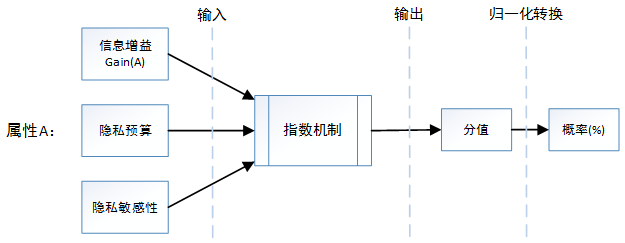
\includegraphics[width=5in]{chap1/diffp-c45}
	\bicaption[fig:diffp-c45]{图}{Diffp-C4.5选择属性的核心计算过程}{Fig.}{The core computational procedure of Diffp-C4.5 in selecting attribute}
\end{figure}

不同于SuLQ ID3和DiffP-C4.5,DiffGen\cite{DiffGen}采用了非交互式框架,并基于指数机制构建分类模型,最后发布匿名化数据集。此算法作为本文优化算法的基础,将在后边章节详细介绍。

\subsection{维度问题}
\label{sec:weidu}
维度(dimension)问题主要指数据集维度和查询维度,在面向数据挖掘应用的差分隐私算法中是个难点问题。假设数据集有d个属性,\{A$_{1}$,A$_{2}$,...,A$_{d}$\},每个属性A$_{i}$(i=1,2,...,d)有|A$_{i}$|个属性值,则它的数据集维度大小为\(\prod\limits_{i = 1}^d {|A{_i} |}\),与属性及属性值个数相关。查询维度指的是查询涉及到的属性个数,最多为d。

为了便于统计、查询,列联表(contingency table)和立方表(Cuboid)是常见的处理方式。如图\ref{fig:cuboid}的示例,在表(a)的原表中有3个属性“性别”,“年龄”和“成绩”,针对不同属性组合下的“计数”的边界查询需求(marginals\cite{marginals}),通常采用空间换时间策略,即枚举各种属性组合生成相应的Cuboid表以达到加速查询的目的,如\ref{fig:cuboid}(b)(c)(d)所示,分别支持查询维度为3,1,2的查询请求。

\begin{figure}[!htp]
	\centering
	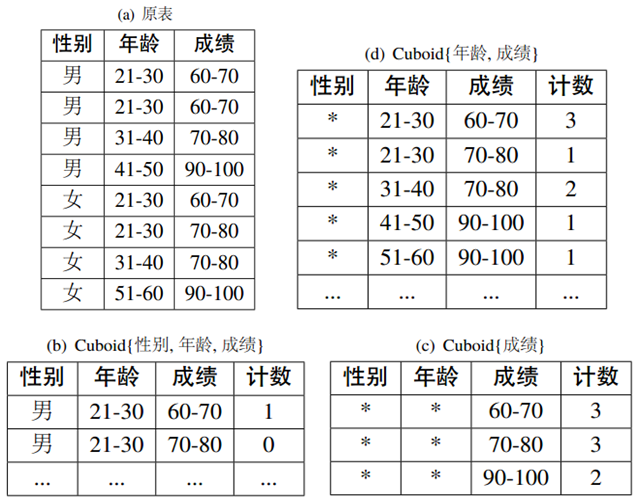
\includegraphics[width=5in]{chap1/cuboid}
	\bicaption[fig:cuboid]{图}{立方表示例}{Fig.}{Sample Cuboid}
\end{figure}

%会随着数据集属性的数量及每个属性的属性值个数的增加而变大
但是这种处理方式在复杂数据表中会由于较大量级的数据集维度和查询维度,引起时间和空间复杂度等问题。若某数据集有10个属性,每个属性有20个属性值,那么它需要维护$2^{10}$-1张Cuboid表,并且最大的一张Cuboid表的表项数等于其维度大小——$20^{10}$。近乎10TB的量级的辅助表不仅在大小上远远超过了原表,并且查询效率低下。但这种维度的数据集在现实情况中很常见。在差分隐私领域中,还会产生许多新问题,本文主要探讨噪音叠加现象——由于查询涉及到的行项数目是和数据维度相关的,因此在较大查询维度请求中差分隐私的噪音会严重积累,影响真实结果。以下对典型的研究工作进行介绍。

Zhang\cite{privbayes}等人提出非交互式差分隐私框架的PrivBayes算法来优化此问题。它借助贝叶斯网络模型,其核心思想是利用具有依赖关系(贝叶斯网络中的条件概率)的低维概率分布来概括具有较高数据维度的原数据集,然后通过在条件概率上加噪的方式替代传统的辅助表行项加噪达到降维目的,最后根据概率模型构建新数据集并发布。

Xiao\cite{wavelet}等人指出,对于范围计数类查询(Range-count query),查询结果的噪音方差是与查询涉及到的行数相关。他们通过小波变换原理给隐私代价设置权值,从减小噪音方差的角度优化拉普拉斯噪音量级,从而达到优化范围查询的目的。

Hay\cite{boosting}等人针对一维无归属直方图(Unattributed Histogram),通过一致性约束(Consistency Constraints)和最小二乘法对噪音的分布进行约束求精。虽然此方法仅支持单位长度的查询请求,但是其一致性约束思想和树状优化结构的使用给基于范围查询的差分隐私噪音优化研究提供了新思路。

\section{论文组织结构}

本文正文共有六章,在归纳研究背景、分析研究现状的基础上,针对分类应用中范围计数查询引起的噪音线性叠加问题,首先揭示经典算法的缺陷模型,接着介绍优化思路并设计实现一种非交互式差分隐私匿名优化算法DiffCon,最后通过真实数据集测试算法性能并讨论实验结果。

本文第二章是问题描述的重点章节。首先介绍差分隐私相关的定义,然后基于频率矩阵加噪模型,对所关注问题进行量化描述。

本文第三章就本课题的核心问题---分类需求中范围计数查询带来的噪音线性叠加问题,详细介绍经典算法并揭示其缺陷模型。

本文第四章就经典算法的缺陷,详细介绍优化算法DiffCon的设计思路和核心算法。

本文第五章为实验实现与分析,介绍相关实验平台、测试数据集和性能指标,总结并分析实验结果。

本文第六章为总结与展望,基于本文提出的方案,介绍其创新性,并在此基础上进一步展望存在的改进点。